\newpage

\section{Implementácia}
\label{implement}
Zdrojový kód môjho riešenia je napísaný v jazyku Python s použitím nasledujúcich hlavných knižníc:
\begin{itemize}
	\item TensorFlow\footnote{https://www.tensorflow.org/} - open-source knižnica pre strojové učenie. Použitá na vytvorenie modelu neurónovej siete a prácu s ňou.
	\item Matplotlib\footnote{https://matplotlib.org/} - knižnica pre 2D vykresľovanie. V mojom riešení je použitá hlavne na výsledné zobrazenie (resp. uloženie) predikovaných máp výraznosti (teplotných máp) na konkrétnom obrázku webovej stránky. 
	\item PIL (Python Image Library\footnote{http://www.pythonware.com/products/pil/}) - knižnica pre prácu s obrázkami. Použitá je hlavne na načítanie obrázkov webových stránok a zmenu ich rozmerov podľa potreby. 
\end{itemize}

Celá implementácia aj spolu s ukážkami zdrojových kódov funkcií je ešte podrobnejšie popísaná v prílohe \ref{technical_documentation}.

\subsection{Spracovanie datasetu pre neurónovú sieť}

Získaný dataset pozostával z 50 obrázkov a pohľadov 20 ľudí na ne. Najprv ho  bolo nutné upraviť k trénovaniu neurónovej siete. Úprava pozostávala zo zmenšenia a zmeny rozlíšenia obrázkov web stránok pre neurónovú sieť na štvorec o veľkosti \textit{a} x \textit{a}. To zabezpečuje funkcia \textit{\textbf{resize\_image (image, size)}}, ktorá ako parametre dostane obrázok a veľkosť (\textit{size = a}), na ktorú má byť obrázok prevedený.

Ďalej bola nutná normalizácia a vyfiltrovanie fixácií, k čomu slúži funkcia \textit{\textbf{load\_fixations (path)}}. Ako argument dostane CSV súbor exportovaných dát z experimentu, ktorý má za úlohu spracovať. Súbor je spracovávaný sekvenčne po riadkoch, pri čom sú ignorované pre nás nepodstatné záznamy, ako napr. pohľady na medzisnímku pre rozhodenie pozornosti. Fixácie mimo obrázka sú rovnako preskočené a každá fixácia je znormalizovaná. Dáta (meno obrázka, fixácie a ich dĺžky) sú potom uložené pre participantov jednotlivo. 

Pre neurónovú sieť je ešte nutné vypočítať mapy výraznosti (teplotné mapy) z vyfiltrovaných fixácií použítím Gaussovho rozdelenia, ktorého rovnica je ukázaná vo vzorci \ref{gauss}. Najprv však bolo nutné prepočítať fixáciu na konkrétny pixel na obrázku, pomocou nasledujúceho vzorca:

\begin{equation}
[x, y] = [fixation\_x * a, fixation\_y * a]
\label{fixation_convert}
\end{equation}

[\textit{x, y}] - bod v obrázku

\textit{a} - veľkosť strany obrázka (keďže je štvorec)

\textit{fixation\_x} - x-ová normalizovaná súradnica fixácie

\textit{fixation\_y} - y-ová normalizovaná súradnica fixácie
\newline

Toto zabezpečilo rovnakú veľkosť obrázkov a prislúchajúcich máp výraznosti k nim. Hodnota Gaussovho rozdelenia je vypočítaná prakticky pre všetky body z fixácií. 

\begin{equation}
f (x \mid  \mu, \sigma^2 ) = \frac{1}{\sqrt {2 \sigma^2 \pi}} * e^{-\frac{(x- \mu )^2}{2\sigma^2}}
\label{gauss}
\end{equation}

\textit{x} - aktuálny bod, pre ktorý je počítané Gaussovo rozdelenie

\((x - \mu )^{2}\) - vzdialenosť medzi bodom a fixáciou

\(\sigma^2\) - dĺžka fixácie
\newline

Obe vyššie uvedené matematické operácie zobrazuje časť kódu na obrázku \ref{fig:fix_gauss_code}.

	\begin{figure}[H]
		
		\begin{center}
			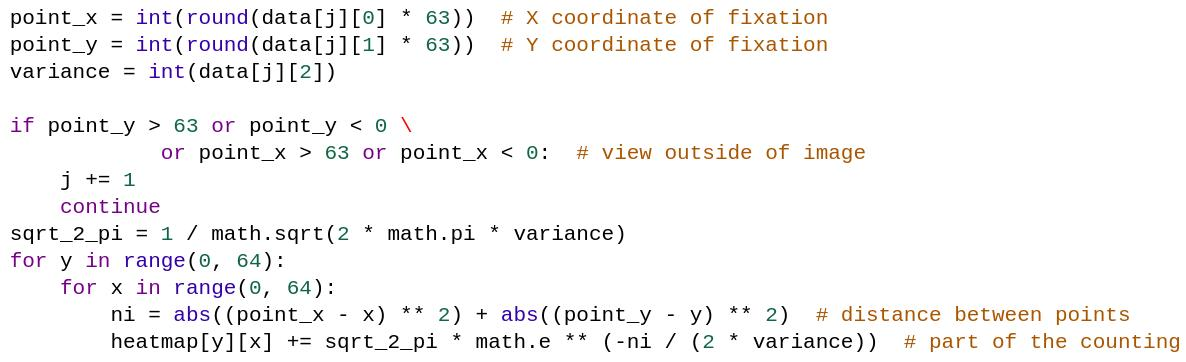
\includegraphics[scale=0.33]{fixations+gauss.jpeg}
		\end{center}
		\caption[Ukážka výpočtu heatmapy]{Ukážka výpočtu heatmapy, kde premenná data obsahuje fixácie a ich dĺžky pre všetky obrázky, heatmap je už konkrétna mapa výraznosti pre obrázok web stránky}
		\label{fig:fix_gauss_code}
	\end{figure}

Kód je súčasťou funkcie \textit{\textbf{load\_coordinates\_for\_image (file\_with\_coordinates, path)}}, ktorej prvý parametrom je súbor s fixáciami participanta a druhým je adresár (cesta) kde sa majú uložiť vypočítané heatmapy. Heatmapy sú ukladané v tvare \textit{heatmap\_i\_image\_j}, kde \textit{i} reprezentuje číslo participanta (začína od nula) a \textit{j} reprezentuje číslo obrázka (od 0 do 49). 

Takto pripravený dataset máp výraznosti pre neurónovú sieť je neskôr rozdelený v pomere 80-10-10 (trénovanie-validácia-testovanie).

\subsection{Trénovanie neurónovej siete}

Trénovanie neurónovej siete prebieha na už spomínaných 80\% dát z datasetu, 10\% je venovaných validácii. Najprv je pomocou funkcie \textit{\textbf{neural\_network\_model (data, keep\_prob)}} vytvorený model siete, ktorého schéma aj s popisom je v Návrhu v časti \ref{navrh}. Parameter \textit{data} predstavuje vstup pre neurónovú sieť, v našom prípade obrázok, resp. obrázky. Parameter \textit{keep\_prob} určuje hodnotu na vrstve výpadku (z angl. dropout layer), tá je pri trénovaní 0.5, pri validácii a testovaní 1.0. 

Po rozdelení datasetu, nastavení krížových entropií (z angl. cross entropy) a optimizéru je neurónová sieť trénovaná v 15 iteráciách po 30 epoch. V každej iterácii sa trénuje a validuje na celom datasete k tomu určenom, ten je však vždy na začiatku náhodne zamiešaný (ako je vidieť v ukážke kódu na obrázku \ref{fig:shuffle_dataset}), neurónová sieť sa teda učí na náhodných dátach a nie vždy na úplne tých istých.  

	\begin{figure}[H]
		
		\begin{center}
			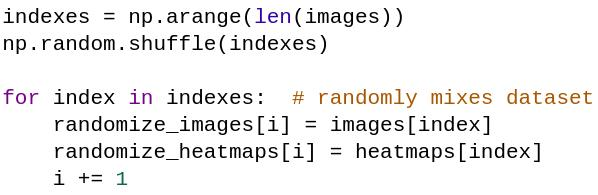
\includegraphics[scale=0.33]{random_dataset.jpeg}
		\end{center}
		\caption[Ukážka náhodného zamiešania datasetu pre trénovanie]{Ukážka náhodného zamiešania datasetu pre trénovanie}\label{fig:shuffle_dataset}
	\end{figure}
	
Vstupom do neurónovej siete je teda séria obrázkov, konkrétne o veľkosti \textit{64x64}. Výstupom sú heatmapy (mapy výraznosti) rovnakej veľkosti. 
	

Trénovanie končí buď po uplynutí všetkých epoch alebo v momente, kedy chyba predikcie na validačnom datasete prestane klesať a začne rásť. To značí, že sieť sa už neučí, ale začína sa pretrénovávať. 

Po tomto bode nasleduje otestovanie neurónovej siete na zvyšných 10\% datasetu a uloženie celého natrénovaného modelu. 

\subsection{Využívanie natrénovaného modelu}
Predikovať heatmapy k novým obrázkom pomocou natrénovaného modelu umožňuje funkcia \ \textit{\textbf{predict(model, directory\_with\_images, directory\_for\_saved\_ predictions, heatmap\_type, metrics\_set=None)}}, ktorá ako parametre dostane spomínaný model, adresár s obrázkami (na ich veľkosti nezáleží), adresár kam sa majú uložiť výsledné predikcie a typ heatmapy, ktorá sa má zobraziť. Ako voliteľný parameter je zvolenie/nezvolenie výpočtu metrík ohodnocujúcich kvalitu predikcií vizuálnej pozornosti. Po predikcii máp výraznosti sa tak v závislosti od voliteľného parametra môžu volať funkcie na výpočet už spomínaných metrík, ktoré sú prevzaté z open-source-ového repozitára\footnote{https://github.com/herrlich10/saliency}. K zobrazeniu/uloženiu predikcií slúži funkcia \textit{\textbf{visualize\_heatmap (heatmap, orig, path\_for\_saving, heatmap\_type)}}, tá má ako parametre heatmapu (teda našu predikciu), originálny obrázok, pre ktorý sa robila predikcia, cestu kam sa má uložiť výsledok a nakoniec typ zobrazovanej heatmapy. 